\documentclass{article}

% Language setting
% Replace `english' with e.g. `spanish' to change the document language
\usepackage[english]{babel}
\usepackage{blindtext}
\usepackage{listings}

\usepackage[most]{tcolorbox}

\newcommand{\SubItem}[1]{
    {\setlength\itemindent{15pt} \item[-] #1}
}
\makeatletter
\NewDocumentCommand{\mynote}{+O{}+m}{%
  \begingroup
  \tcbset{%
    noteshift/.store in=\mynote@shift,
    noteshift=1.5cm
  }
  \begin{tcolorbox}[nobeforeafter,
    enhanced,
    sharp corners,
    toprule=1pt,
    bottomrule=1pt,
    leftrule=0pt,
    rightrule=0pt,
    colback=yellow!20,
    #1,
    left skip=\mynote@shift,
    right skip=\mynote@shift,
    overlay={\node[right] (mynotenode) at ([xshift=-\mynote@shift]frame.west) {\textbf{Note:}} ;},
    ]
    #2
  \end{tcolorbox}
  \endgroup
  }
\makeatother


% Set page size and margins
% Replace `letterpaper' with `a4paper' for UK/EU standard size
\usepackage[letterpaper,top=2cm,bottom=2cm,left=2cm,right=2cm,marginparwidth=1cm]{geometry}

% Useful packages
\usepackage{amsmath}
\usepackage{graphicx}
\usepackage[colorlinks=true, allcolors=blue]{hyperref}

\title{How To Use PLaF With Github}
\author{Sarang Hadagali \\ Version 1}

\begin{document}
\maketitle

\section{Why Github}

Using Github to access and modify the PLaF folder is great beacuse it allows you to save your work on an online repository that won't be deleted if something goes wrong on your computer. You are also very easily able to update your folder if Professor ever decides to make changes to it. \\


\mynote{Create and setup a Github account before completeing the rest of this. Also you have to delete any local PLaF copies you have before starting this, so if you have any work on the PLaF directory make sure to save it and then copy it in later!}

\subsection{Cloning vs. Forking}
There are two options when using Github, you could either clone the repository or fork it. Cloning the repository tends to be easier as there are less steps, however, there are limitations that you will experience as we do not have push access to the origin repo. For example, when cloning if you make edits on your local copy and then want to pull from Professor's origin branch then you may have to stash your changes which can cause headaches to get back. A better solution is to fork the repository, which is the same thing as cloning but with an extra step. Forking the repo, allows you to make a new duplicate repo that is still connected to the Professor's original branch but also allows you to push and save your changes at the same time, avoiding the issue of stashing your changes.


\section{Forking Setup}
\subsection{Forking PLaF}
\begin{enumerate}
    \item Open up the \href{https://github.com/ebonelli/PLaF}{PLaF} repo and in the top right corner of the screen select Fork 
    \item Title your repo whatever you'd like, you can just leave it PLaF
    \item Leave the default setting selected and click "create fork"
    \item You should now be in a screen that has "you github username"/PLaF as opposed to ebonelli/PLaF
    \item Select the green "Code" button \\
    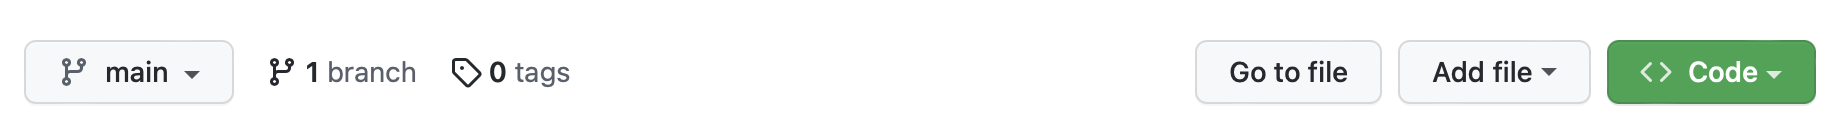
\includegraphics[width=1\textwidth]{images/codeButton.png}
    \item Select "HTTPS" and copy the link "https://github.com/"YOUR-USERNAME"/PLaF.git
    \item Navigate to a terminal and cd into the folder you want to create your PLaF folder in
    \item Type "git clone" and paste the link you just copied \\ \\
    \centerline{
\includegraphics[width=1\textwidth]{images/clone.png}}
    \item Enter and then cd into the PLaF folder
    \SubItem{Enter "ls" and you should be able to see the PLaF folder within your directory}
\end{enumerate}

\subsection{Setting Up Local Git Repository}
Now that we have the PLaF folder we can move onto setting up the local git repository that will allow us to push and pull the new Github repo without effecting the Professor's repo. \\

In your PLaF folder type "git remote -v" 
\begin{verbatim}
    terminal@your-terminal PLaF % git remote -v
    origin https://github.com/"githubUsername"/PLaF.git (fetch)
    origin https://github.com/"githubUsername"/PLaF.git (push)
\end{verbatim}

% \noindent
% \begin{lstlisting}[language=bash]
%   # Initialize git repo
%   $ git init
%   # Adds all files that were changed
%   $ git add .
%   # Commits the changes you have made with a message
%   $ git comit -m "first commit"
%   # Switches to main branch
%   $ git branch -M main
%   # Pushes changes to main
%   $ git push -u origin main
% \end{lstlisting}



\subsection{Setting Upstream}
The next part linking this to the upstream repo, AKA, the Professors repo. Follow the code snippet below in your PLaF directory

\begin{verbatim}
    $ git remote add upstream https://github.com/ebonelli/PLaF.git
    $ git pull upstream main
\end{verbatim}
  
Once again run "git remote -v" your output should now be 
\begin{verbatim}
    terminal@your-terminal PLaF % git remote -v
    origin https://github.com/"githubUsername"/PLaF.git (fetch)
    origin https://github.com/"githubUsername"/PLaF.git (push)
    upstream       https://github.com/ebonelli/PLaF.git (fetch)
    upstream       https://github.com/ebonelli/PLaF.git (push)
    
\end{verbatim}

Congratulations You have now set up a forked repository!

\subsection{Login to Github}
If you are using a virtual machine or have never used github before locally then you may encounter an issue when trying to push something. If you are prompted with "git config —global user.email" and "git config —global user.name" just input the email you signed up with github and your github user name. If your terminal output asks for username and password follow the steps below. If not you can skip this step. \\

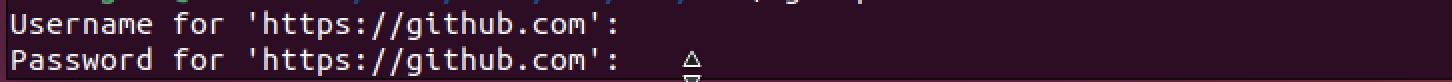
\includegraphics[width=1\textwidth]{images/errorLogin.png} \\ 

\begin{enumerate}
    \item Enter your normal github username and press enter
    \SubItem{Do not type in your password this will not work as Github has changed its security policy and now requires a special token}
    \item Go to github and navigate to settings
    \item Scroll to the bottom of the page and select developer settings on the left sidebar \\
    \item Select the Personal access tokens drop down
    \item Select the second option Tokens(classic) \\
    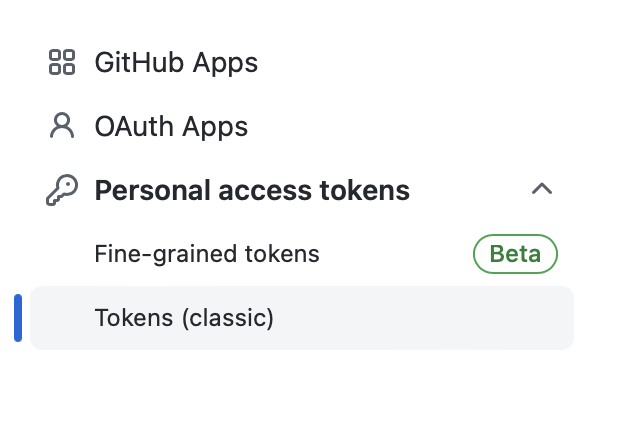
\includegraphics[width=.5\textwidth]{images/tokens.png} 
    \item Click generate new token at the top
    \item Select the second option "Generate new token(classic)"
    \item You can type in some note that explains what you are using it for such as "PLaF Access"
    \item You can set the expiration date to however long you want, but if you set it up too short then you may have to redo these steps in the future
    \item Since this is a repo for yourself you can select all the permissions that are given
    \item You should now have a long generated token, copy this and paste it into the password field
    \item You should have access to your github repo locally now, and should be able to push and pull.
\end{enumerate}

\noindent
With this you should be able to push to your repo. Make sure to keep this token safe as github will not display it once you close the tab so you will have to redo this if you don't copy it somewhere.

\section{How to Use}
Now that you have created your own forked repo that is connected to the Professors repo here are a couple of pointers on how to effectively use git.
\begin{itemize}
    \item To push your changes to your remote repository first make sure you are on your main branch by typing "git branch" and there should be *main outputted then
    \begin{verbatim}
        $ git add .
        $ git commit -m "new commit"
        $ git push origin main 
    \end{verbatim}
    \item If Professor ever asks you to pull from the repo, first follow the step mentioned above to push your changes then do
        \SubItem{git pull upstream main}
        \SubItem{This should automatically merge your changes with the new changes that Professor has added. However if you have merge conflicts you are going to have to manually resolve that.}
\end{itemize}

\noindent
If you are having any issues with forking follow this Stack Overflow \href{https://stackoverflow.com/questions/3903817/pull-new-updates-from-original-github-repository-into-forked-github-repository}{post} as this is what I used to figure it out. \\

\noindent
Everything should be working now and you can continue with the normal process of dune build and dune install. Hopefully the process wasn't too bad and you learned a thing or two about working with Git/Github. There are a lot more features to git so check them out it is a useful skill to have as a CS major!
Also feel free to add onto this! The link to this repo is \href{https://github.com/shadagali03/How_To_Github_PLaF}{here}. If you find any mistakes or any ways to improve it create your own branch and make a pull request and I can take a look at it. Good luck!
\end{document}